\documentclass[a4paper,12pt]{article}
\usepackage[czech]{babel}
\usepackage[utf8]{inputenc}
\usepackage{amsmath}
\usepackage[bookmarksopen,colorlinks,plainpages=false,urlcolor=blue]{hyperref}


\usepackage{url}

\usepackage{ifpdf}

\ifpdf
  \usepackage[dvipdf]{graphicx}
\else
  \usepackage[dvips]{graphicx}
\fi

\usepackage[top=2cm, left=2cm, text={17cm, 26cm}, ignorefoot]{geometry}
\author{David Kolečkář - xkolec07}
\title{ITO}
%Zacatek dokumentu
\begin{document}

\begin{figure}[!h]
  \centering
  
\includegraphics[height=5cm]{logo}
\end{figure}

\begin{center}
\bigskip
\begin{Huge}
Teorie obvodů 2014/2015\\
\end{Huge}
\begin{large}
Projekt
\end{large}
\end{center}

\begin{center}
\begin{Large}
\today
\end{Large}
\end{center}

\vfill

\begin{flushleft}
\begin{large}
\begin{tabular}{ll}
Autor: & David Kolečkář, \url{xkolec07@stud.fit.vutbr.cz} \\
 & Fakulta Informačních Technologií \\
 & Vysoké Učení Technické v~Brně \\
\end{tabular}
\end{large}
\end{flushleft}

% % % % % % % % % % % % % % % % % % % % % % % % % % % % % % % % % % % % % % % % % % % % % % % %
\newpage
\begin{center}
\textbf{Příklad 1, Varianta D}
\end{center}
\bigskip
Stanovte napětí
\textcolor{red}{$U_{R7}$}
a proud
\textcolor{red}{$I_{R7}$}.
Použijte metodu postupného zjednodušování obvodu.
\bigskip

Zadané hodnoty

%%%%%%%%%%%    TABULKA    %%%%%%%%%%
\begin{tabular} {|  c | c | c | c | c | c | c | c | c | }
\hline
U[V] & $R_1[\Omega]$ & $R_2[\Omega]$ & $R_3[\Omega]$ & $R_4[\Omega]$ & $R_5[\Omega]$ & $R_6[\Omega]$ & $R_7[\Omega]$ & $R_8[\Omega]$\\ \hline
105 & 420 & 980 & 330 & 280 & 310 & 710 & 240 & 200 \\ \hline
\end{tabular}
\bigskip
%%%%%%%%%%%    TABULKA    %%%%%%%%%%


%%%%%%%%%%%    ZADANI    %%%%%%%%%%
\begin{center}
\includegraphics[height=7cm]{pr1/dia}
\end{center}

\bigskip
1.Obvody $R_5$ a $R_6$ jsou zapojeny paralelně. Spočítáme je.
\begin{equation*}
R_{56} = \frac{R_5 * R_6}{ R_5 + R_6} = \frac{310\ \Omega*710\ \Omega}{310\ \Omega+710\ \Omega} = 215,7843\ \Omega
\end{equation*}
\bigskip

2. Obvod transfigurujeme na hvězdu
%%%%%%%%%%%    HVEZDA    %%%%%%%%%%

\begin{center}
\includegraphics[height=5cm]{pr1/pr1gr2}
\end{center}

\newpage

\begin{equation*}
R_A = \frac{R_2 * R_3}{ R_2 + R_3 + R_4} = \frac{420\ \Omega*330\ \Omega}{420\ \Omega+330\ \Omega+280\ \Omega} = 203,3962\ \Omega
\end{equation*}
\begin{equation*}
R_B = \frac{R_2 * R_4}{ R_2 + R_3 + R_4} = \frac{420\ \Omega*280\ \Omega}{420\ \Omega+330\ \Omega+280\ \Omega} = 172,5786\ \Omega
\end{equation*}
\begin{equation*}
R_C = \frac{R_3 * R_4}{ R_2 + R_3 + R_4} = \frac{330\ \Omega*280\ \Omega}{420\ \Omega+330\ \Omega+280\ \Omega} = 58,1132\ \Omega
\end{equation*}


\bigskip
3.Nyní sečteme rezistory, které jsou zapojeny sériově. Tedy $R_1$ a $R_A$, $R_B$ a $R_{56}$, $R_C$ a $R_7$
\begin{center}
\includegraphics [height=5cm]{pr1/serie}
\end{center}
\bigskip
\begin{equation*}
R_{A1} = R_A + R_1 = 203,3962\ \Omega + 420\ \Omega = 623,3962\ \Omega
\end{equation*}
\begin{equation*}
R_{B56} = R_B + R_{56} = 172,5786\ \Omega + 215,7843\ \Omega = 388,3629\ \Omega
\end{equation*}
\begin{equation*}
R_{C7} = R_C + R_7 = 58,1132\ \Omega + 240\ \Omega = 298,1132\ \Omega
\end{equation*}





\bigskip

4.A poté sečteme paralelně zapojené rezistory $R_{B56}$ a $R_{C7}$ a výsledný odpor $R_{BC567}$ sečteme s rezistorem $R_{A1}$ a $R_8$. Dostáváme $R_{EKV}$.
\begin{center}
\includegraphics [height=5cm]{pr1/paralelne}
\end{center}
\begin{equation*}
R_{BC567} = \frac{ R_{B56} * R_{C7}}{R_{B56} + R_{C7}} = \frac{298,1132\ \Omega*388,3629\ \Omega}{298,1132\ \Omega+388,3629\ \Omega} = 168,6528\ \Omega
\end{equation*}
\begin{equation*}
R_{EKV} = R_{A1} + R_{BC567} + R_8 = 623,3962\ \Omega + 168,6528\ \Omega = 200\ \Omega = 992,049\ \Omega
\end{equation*}

\begin{center}
\includegraphics [height=5cm]{pr1/rekv}
\end{center}
\newpage

5. Vypočítáme proud $I$

\begin{equation*}
I = \frac{U}{R_{EKV}} = \frac{105\ V}{992,049\ \Omega} = 0,1058\ A
\end{equation*}

6. Vypočítáme napětí $U_{BC567}$ 

\begin{equation*}
U_{BC567} = R_{BC567} * I = 168,6528\ \Omega * 0,1058\ A = 17,8505 \ V
\end{equation*}


7. Dále vypočítáme proud $I_{R7}$ 
\begin{equation*}
I_{R7} = \frac{U_{BC567}}{R_{C7}} = \frac{17,8505 \ V}{298,1132\ \Omega} = 0,0599\ A
\end{equation*}


8. Nakonec vypočítáme napětí $U_{R7}$
\begin{equation*}
U_{R7} = R_7 * I_{R7} = 240\ \Omega * 0,0599\ A = 14,376\ V
\end{equation*}

\newpage

% % % % % % % % % %  2. Priklad % % % % % % % % % % % % % % % % % % % % % % % % 
\begin{center}
\textbf{Příklad 2, Varianta H}
\end{center}
\bigskip
Stanovte napětí
\textcolor{red}{$U_{R3}$}
a proud
\textcolor{red}{$I_{R3}$}.
Použite metodu Theveninovy věty.
\bigskip

Zadané hodnoty

\begin{tabular} {|  c | c |  c | c | c | c | c |}
\hline
U[V] & $R_1[\Omega]$ & $R_2[\Omega]$ & $R_3[\Omega]$ & $R_4[\Omega]$ & $R_5[\Omega]$ & $R_6[\Omega]$\\ \hline
220 & 360 & 580 & 205 & 560 & 350 & 300 \\ \hline
\end{tabular}
\bigskip

\begin{center}
\includegraphics[height=5cm]{pr2/pr2gr1.eps}
\end{center}

1. Vypočítame $R_{EKV}$ pomocí hvězdy

\begin{center}
\includegraphics[height=5cm]{pr2/pr2gr3}
\end{center}

\begin{equation*}
R_X = \frac{R_1*R_2}{R_1+R_2+R_3} = \frac{360\ \Omega*580\ \Omega}{360\ \Omega + 580\ \Omega + 205\ \Omega} = 182,3581\ \Omega
\end{equation*}

\begin{equation*}
R_Y = \frac{R_1*R_3}{R_1+R_2+R_3} = \frac{360\ \Omega*205\ \Omega}{360\ \Omega + 580\ \Omega + 205\ \Omega} = 64,4541\ \Omega
\end{equation*}

\begin{equation*}
R_Z = \frac{R_2*R_3}{R_1+R_2+R_3} = \frac{580\ \Omega*205\ \Omega}{360\ \Omega + 580\ \Omega + 205\ \Omega} = 103,8427\ \Omega
\end{equation*}

\begin{equation*}
R_{Y4} = 64,4541\ \Omega + 560\ \Omega = 624,4541\ \Omega 
\end{equation*}

\begin{equation*}
R_{Z5} = 103,8427\ \Omega + 350\ \Omega = 453,8427\ \Omega 
\end{equation*}

\begin{equation*}
R_{YZ45} = \frac{R_{Y4}*R_{Z5}}{R_{Y4}+R_{Z5}} = \frac{624,4541\ \Omega* 453,8427\ \Omega}{624,4541\ \Omega + 453,8427\ \Omega} = 262,8255\ \Omega
\end{equation*}

\begin{equation*}
R_{EKV} = R_X + R_{YZ45} + R_6 = 745,1836\ \Omega
\end{equation*}

2. Vypočítáme celkový proud v obvodu

\begin{equation*}
I = \frac{U}{R_{EKV}} = \frac{220 V}{745,1836\ \Omega} = 0,2952\ A
\end{equation*}

3. Zkratujeme $R_3$ a zjednodušíme:

\begin{center}
\includegraphics[height=5cm]{pr2/pr2gr4}
\end{center}

4. Zjednodušený obvod upravíme na hvězdu a vypočítáme $R_i$

\begin{center}
\includegraphics[width= 8cm]{pr2/pr2gr5}
\end{center}

\begin{equation*}
R_X = \frac{R_1*R_4}{R_1+R_4+R_6} = \frac{360\ \Omega * 560\ \Omega}{360\ \Omega + 560\ \Omega + 300\ \Omega} = 165,2459\ \Omega
\end{equation*}

\begin{equation*}
R_Y = \frac{R_1*R_6}{R_1+R_4+R_6} = \frac{360\ \Omega * 300\ \Omega}{360\ \Omega + 560\ \Omega + 300\ \Omega} = 88,5245\ \Omega
\end{equation*}

\begin{equation*}
R_Z = \frac{R_4*R_6}{R_1+R_4+R_6} = \frac{560\ \Omega * 300\ \Omega}{360\ \Omega + 560\ \Omega + 300\ \Omega} = 137,7049\ \Omega
\end{equation*}

\begin{equation*}
R_{Y2} = R_Y + R_2 = 88,5245\ \Omega + 580\ \Omega = 668,5245\ \Omega
\end{equation*}

\begin{equation*}
R_{Z5} = R_Z + R_5 =  137,7049\ \Omega + 350\ \Omega = 487,7049\ \Omega
\end{equation*}

\begin{equation*}
R_{ZY25} = \frac{R_{Y2}*R_{Z5}}{R_{Y2}+R_{Z5}} = \frac{668,5245\ \Omega*487,7049\ \Omega}{668,5245\ \Omega + 487,7049\ \Omega} = 281,9878\ \Omega
\end{equation*}

\begin{equation*}
R_{i} = R_{ZY25} + R_X =  281,9878\ \Omega + 165,2459\ \Omega = 447,2338\ \Omega
\end{equation*}
\newpage
5. Dále vypočítáme napětí $U_i$ 

\begin{center}
\includegraphics[height=5cm]{pr2/pr2gr6}
\end{center}

\begin{equation*}
R_1 * I_X + R_4 * I_X + R_6 * I - U = 0
\end{equation*}
\begin{equation*}
R_2 * I_Y + R_5 * I_Y + R_6 * I - U = 0
\end{equation*}
\begin{equation*}
R_1 * I_X + U_i - R_2 * I_Y = 0
\end{equation*}

\begin{equation*}
I_X = \frac{U - R_6 * I}{R_1 + R_4} = \frac{220\ U - 300\ \Omega * 0,2952\ I}{360\ \Omega + 560\ \Omega} = 0,1428\ A
\end{equation*}

\begin{equation*}
I_Y = \frac{U - R_6 * I}{R_2 + R_5} = \frac{220\ U - 300\ \Omega * 0,2952\ I}{580\ \Omega + 350\ \Omega} = 0,1413\ A
\end{equation*}


\begin{equation*}
U_i = R_2 * I_Y - R_1 * I_X = 580\ \Omega * 0,1413\ A - 360\ \Omega * 0,1428\ A  = 30,546\ V
\end{equation*}

6. Vytvoříme ekvivalentní obvod a vypočítáme $I_{R3}$ a $U_{R3}$ 

\begin{center}
\includegraphics[height=5cm]{pr2/pr2gr2}
\end{center}

\begin{equation*}
I_{R3} = \frac{U_i}{R_i + R_3} = \frac{30,546\ V}{447,2338\ \Omega + 205\ \Omega} = 0,05449\ A 
\end{equation*}

\begin{equation*}
U_{R3} = R_3 * I_{R3} = 205\ \Omega * 0,05449\ A = 11,1704\ V
\end{equation*}

\newpage

% % % % % % % % % %  3. Priklad % % % % % % % % % % % % % % % % % % % % % % % % 
\begin{center}
\textbf{Příklad 3, Varianta F}
\end{center}
\bigskip

Stanovte napětí \textcolor{red}{$U_{R_5}$} a proud \textcolor{red}{$I_{R_5}$}.
Použijte metodu uzlových napětí ($U_a$, $U_b$, $U_c$).\\

\begin{tabular} {| c | c | c | c | c | c | c | c | c | }
\hline
 $U_1[V]$
&$U_2[V]$
&$I[A]$
&$R_1[\Omega]$
&$R_2[\Omega]$
&$R_3[\Omega]$
&$R_4[\Omega]$
&$R_5[\Omega]$
&$R_6[\Omega]$
\\ \hline

145 & 75 & 0,85 & 480 & 440 & 530 & 360 & 255 & 190 \\ \hline

\end{tabular}

\begin{center}
\includegraphics[height=6cm]{pr3/pr3gr3}
\end{center}

1. Stanovíme rovnice pro jednotlivé uzly
\begin{align*}
A :& I_{R_1} - I - I_{R_2} - I_{R_3} = 0\\
B :& I_{R_3} + I - I_{R_5} + I_{R_6} = 0\\
C :& I_{R_5} - I_{R_6} - I_{R_4} = 0
\end{align*}

2. Vyjádříme jednotlivé proudy

$$
I_{R_1} = \cfrac{U_1 - U_A}{R_1}\qquad
I_{R_2} = \cfrac{U_A}{R_2}\qquad
I_{R_3} = \cfrac{U_A - U_B}{R_3}
$$
$$
I_{R_4} = \cfrac{U_C}{R_4}\qquad
I_{R_5} = \cfrac{U_B - U_C}{R_5}\qquad
I_{R_6} = \cfrac{U_C - U_B + U_2}{R_6}
$$

3. Dosadíme do rovnice
\begin{align*}
A :& \cfrac{145 - U_A}{480} - 0,85 - \cfrac{U_A}{440} - \cfrac{U_A - U_B}{530} = 0\\
B :& \cfrac{U_A - U_B}{530} + 0,85 - \cfrac{U_B - U_C}{255} + \cfrac{U_C - U_B + 75}{190} = 0\\
C :& \cfrac{U_B - U_C}{255} - \cfrac{U_C - U_B + 75}{190} - \cfrac{U_C}{360} = 0
\end{align*}


4. Vyřešíme rovnice o třech neznámých
\[U_A = -19,7673\ V\]
\[U_B = 224,9912\ V\]
\[U_C = 139,7489\ V\]

5. Vypočítáme požadované hodnoty
\[I_{R_5} = \cfrac{U_B - U_C}{R5} = \cfrac{224,9912\ V - 139,7489\ V}{255\ \Omega} = 0,3343\ A\]
\[U_{R_5} = R_5 * I_{R_5} = 255\ \Omega * 0,3343\ A = 85,2424\ V\]


%\bigskip
\newpage

% % % % % % % % % %  4. Priklad % % % % % % % % % % % % % % % % % % % % % % % % 
\begin{center}
\textbf{Příklad 4, Varianta D}
\end{center}
\bigskip
Pro napájecí napětí platí: $u = U * \sin (2\pi ft)$.\\
Ve vztahu pro napětí $u_{L_2} = U_{L_2} * \sin (2\pi ft + \varphi_{L_2})$ určete $|U_{L_2}|\ a\ \varphi_{L_2}$.
Použíjte metodu zjednodušování obvodu.\\
Pozn: Pomocný směr šipky napájecího zdroje platí pro speciální časový okamžik $(t = \frac{\pi}{2\omega})$.
\bigskip

Zadané hodnoty

\begin{tabular} {|  c | c |  c | c | c | c | c | c | c | }
\hline
U[V] &  $R_1 [\Omega]$  & $R_2 [\Omega]$  &$R_3 [\Omega]$  & $L_1 [mH]$ & $L_2 [mH]$ & $C_1[\mu F]$ & $C_2[\mu F]$  & f [Hz] \\ \hline
50 & 190 & 180 & 220 & 420 & 270 & 120 & 205 & 90\\ \hline
\end{tabular}
\bigskip

\begin{center}
\includegraphics[height=5cm]{pr4/pr4}
\end{center}

1. Výpočet úhlové rychlosti.

$$
\omega = 2\pi f = 565,4862\ rad/s
$$

2. Výpočet induktancí a kapacitancí

$$
 X_{C1} = \cfrac{-j}{\omega * C_1} = \cfrac{-j}{565,4862 * 120 * 10^{-6}} = -14,7492j\ \Omega 
$$
$$
 X_{C2} = \cfrac{-j}{\omega * C_2} = \cfrac{-j}{565,4862 * 205 * 10^{-6}} = -8,6281j\ \Omega
$$

$$
\ X_{L1} = j\omega * L_1 = 565,4862 * 0,42  = 237,5042j\ \Omega 
$$
$$
\ X_{L2} = j\omega * L_2 = 565,4862 * 0,27  = 152,6812j\ \Omega
$$

3. Sériově spojíme $R_{2}$ a $X_{C1}$, $R_{3}$ a $X_{C2}$


$$Z_1 = R_2 + X_{C1} = 180 - 14,7492j\ \Omega$$
$$Z_2 = R_3 + X_{C2} = 220 - 8,6281j\ \Omega$$

4. Paralelně spojíme $Z_{2}$ a $X_{L2}$, $Z_{1}$ a $Z_{3}$
\begin{center}
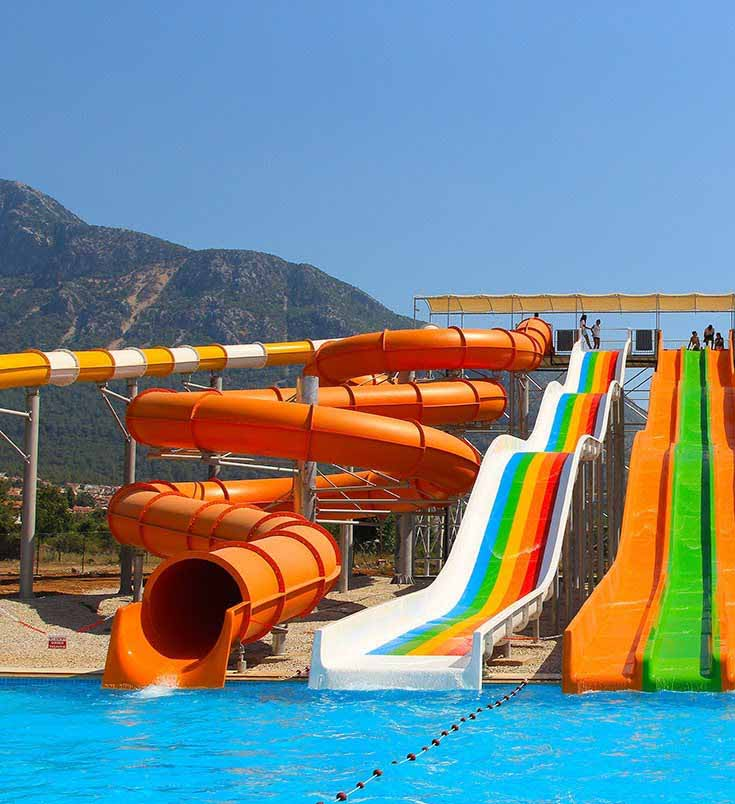
\includegraphics[height=5cm]{pr4/1}
\end{center}
$$ Z_{3} = \cfrac{Z_{2} * X_{L2}}{Z_{2} + X_{L2}} = \cfrac{(220 - 8,6281j) * (152,6812j)}{(220 - 8,6281j) + (152,6812j)} = 74,1336 + 104,1194j\ \Omega$$

\begin{center}

\includegraphics[height=5cm]{pr4/2}
\end{center}

$$ Z_{4} = \cfrac{Z_{3} * Z_{1}}{Z_{3} + Z_{1}} = \cfrac{(74,1336 + 104,1194j) * (180 - 14,7492j)}{(74,1336 + 104,1194j) + (180 - 14,7492j)} = 73,8465 + 43,4679j\ \Omega$$

5. Sériově spojíme $R_{1}$, $Z_{4}$, $X_{L1}$
\begin{center}
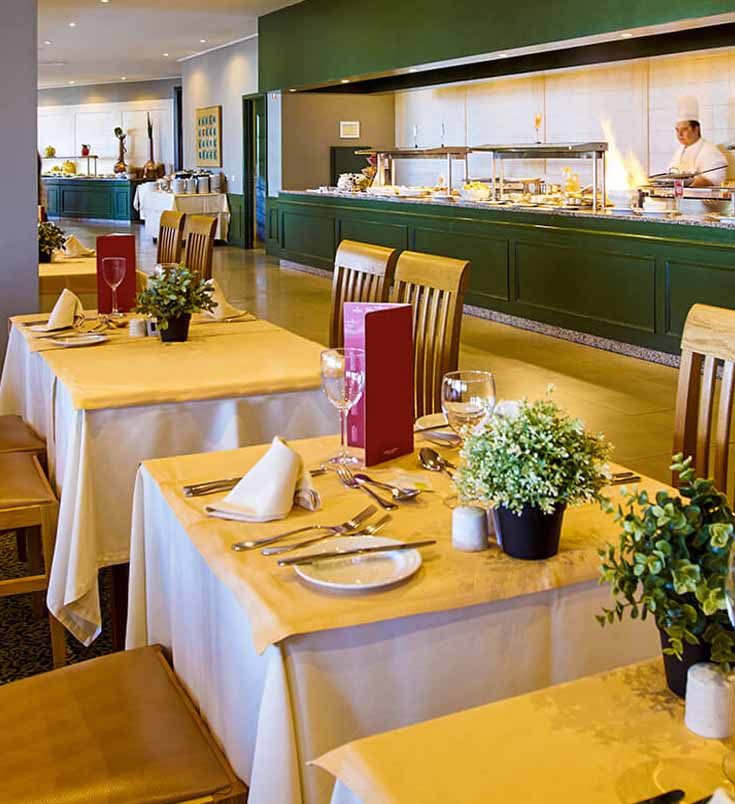
\includegraphics[height=5cm]{pr4/3}
\end{center}
$$
Z = R_1 + Z_4 + X_{L1} = 190 + (73,8465 + 43,4679j) + 237,5042j = 263,8465 + 280,9723j\ \Omega
$$

6. Výpočet celkového proudu

$$
I = \cfrac{U}{Z} = \cfrac{50}{263,8465 + 280,9723j} = 0,0888 - 0,0945j\ A 
$$

7. Výpočet napětí $U_{Z4}$, proud $I_{L2}$ a $U_{L2}$

$$
U_{Z4} = I * Z_4 = (0,0888 - 0,0945j) * (73,8465 + 43,4679j) = 10,6681 - 3,1232j\ V
$$

$$
I_{L2} = \cfrac{U_{Z4}}{X_{L2}} = \cfrac{10,6681 - 3,1232j}{152,6812j} = -0,0205 - 0,0698j\ A 
$$

$$
U_{L2} = U_{Z4}  = 10,6681 - 3,1232j\ V
$$

$$|U_{L2}| = sqrt(10,6681^2 + (- 3,1232)^2) = 11,1159\ V$$
$$\varphi_{L2} = arctan \left|\frac{komplexni}{realna}\right| = arctan \left|\frac{- 3,1232}{10,6681}\right| = -0,2848 rad = -16,3183^\circ$$

\newpage


% % % % % % % % % %  5. Priklad % % % % % % % % % % % % % % % % % % % % % % % % 
\begin{center}
\textbf{Příklad 5, Varianta H}
\end{center}
\bigskip
Pro napájecí napětí platí: $u_1 = U_1 * \sin (2\pi ft)$, $u_2 = U_2 * \sin (2\pi ft)$.\\
Ve vztahu pro napětí $u_{C_1} = U_{C_1} * \sin (2\pi ft + \varphi_{C_1})$ určete $|U_{C_1}|\ a\ \varphi_{C_1}$.\\\\
Použijte metodu smyčkových proudů.
Pozn: Pomocné "směry šipek napájecích zdrojů platí pro speciální časový okamžik $(t = \frac{\pi}{2\omega})$."
\bigskip

Zadané hodnoty

\begin{tabular} {|  c | c | c |  c | c | c | c | c | c | c | }
\hline
$U_1 [V]$ & $U_2 [V]$ &  $R_1 [\Omega]$  & $R_2 [\Omega]$  &$R_3 [\Omega]$  & $L_1 [mH]$ & $L_2 [mH]$ & $C_1[\mu F]$ & $C_2[\mu F]$  & f [Hz] \\ \hline
65 & 60 & 100 & 105 & 145 & 160 & 75 & 155 & 70 & 95\\ \hline
\end{tabular}
\bigskip

\begin{center}
\includegraphics[height=6cm]{pr5/pr5gr1}
\end{center}

1. Výpočet úhlové rychlosti.

$$
\omega = 2\pi f = 596,9021\ rad/s
$$

2. Výpočet induktancí a kapacitancí

$$
 X_{C1} = \cfrac{-j}{\omega * C_1} = \cfrac{-j}{596,9021 * 155 * 10^{-6}} = -10,8108j\ \Omega 
$$
$$
 X_{C2} = \cfrac{-j}{\omega * C_2} = \cfrac{-j}{596,9021 * 70 * 10^{-6}} = -23,9808j\ \Omega
$$

$$
X_{L1} = j\omega * L_1 = 596,9021 * 0,16  = 95,5043j\ \Omega 
$$
$$
X_{L2} = j\omega * L_2 = 596,9021 * 0,075  = 44,7676j\ \Omega
$$
\newpage
3. Sestavíme rovnice pro jednotlivé smyčkové proudy

\begin{center}
\includegraphics[height=6cm]{pr5/pr5gr2}
\end{center}

$$I_{A}: R_{1}I_{A} + U_{1} + X_{C_{2}}(I_{A}-I_{C}) + R_{2}(I_{A}-I_{B})+X_{C_{1}}(I_{A}-I_{B})=0$$
$$I_{B}: X_{C_{1}}(I_{B}-I_{A}) + R_{2}(I_{B}-I_{A}) + X_{L_{2}}(I_{B}-I_{C}) + X_{L_{1}}I_{B}=0$$
$$I_{C}: X_{C_{2}}(I_{C}-I_{A}) + R_{3}I_{C} + U_{2} + X_{L_{2}}(I_{C}-I_{B})=0$$

4. Zjednodušíme

$$(R_{1}+R_{2}+X_{C_{1}}+X_{C_{2}})I_{A} - (R_{2}+X_{C_{1}})I_{B} + X_{C_{2}}I_{C} + U_{1}=0$$
$$(R_{2}+X_{C_{1}}+X_{L_{1}}+X_{L_{2}})I_{B} - (R_{2}+X_{C_{1}})I_{A} - X_{L_{2}}I_{C}=0$$
$$(R_{3}+X_{C_{2}}+X_{L_{2}})I_{C} - X_{C_{2}}I_{A} - X_{L_{2}}I_{B} + U_{2}=0$$

5. Dosadíme hodnoty a vypočítáme $I_{A}, I_{B}, I_{C}$ 

$$(100+105+(-10,8108j)+(-23,9808j))I_{A} - (105+(-10,8108j))I_{B} + (-23,9808j)I_{C} + 65=0$$
$$(105+(-10,8108j)+(95,5043j)+(44,7676j))I_{B} - (105+(-10,8108j))I_{A} - (44,7676j)I_{C}=0$$
$$(145+(-23,9808j)+(44,7676j))I_{C} - (-23,9808j)I_{A} - (44,7676j)I_{B} + 60=0$$

$$I_{A} = -0,4176 + 0,0903j\ A$$
$$I_{B} = -0,2022 + 0,1916j\ A$$
$$I_{C} = -0,4478 + 0,0708j\ A$$

6. Vypočítáme napětí $|U_{C1}|\ a\ \varphi_{C1}$

$$U_{C1} = X_{C_{1}}(I_{A} - I_{B})$$
$$U_{C1} = (-10,8108j) * [(-0,4176 + 0,0903j) - (-0,2022 + 0,1916j)]$$
$$U_{C1} = 1,0949 - 2,3280j\ \ V$$

$$|U_{C1}| = sqrt(1,0949^2 + (- 2,3280)^2) = 2,5726\ V$$
$$\varphi_{C1} = arctan \left|\frac{komplexni}{realna}\right| = arctan \left|\frac{- 2,3280}{1,0949}\right| = -1,1311 rad = -64,8109^\circ$$

\newpage
% % % % % % % % % %  6. Priklad % % % % % % % % % % % % % % % % % % % % % % % % 
\newpage
\begin{center}
\textbf{Priklad 6, Varianta F}
\end{center}
\bigskip
Sestavte diferencialní rovnici popisující chovaní obvodu na obrázku, dále ji upravte dosazením hodnot parametrů. Vypočítejte analytické řešení $i_K = f(t)$. Proveďte kontrolu výpočtu dosazením do sestavené diferencialní rovnice.
\bigskip

Zadané hodnoty

\begin{tabular} {| c | c | c | c |}
\hline
  U [V]
& L [R]
& R [$\Omega$] 
& $i_L(0)$ [A] \\ \hline

9 & 35 & 15 & 4\\ \hline
\end{tabular}
\bigskip


\begin{center}
\includegraphics[height=5cm]{pr6/pr6gr1.eps}
\end{center}

$$i'_L = \cfrac{u_L}{L}$$
$$u_R + u_L - U = 0$$
$$u_L  = U-u_R$$
$$u_L  = U-R * i_L$$
$$i'_L = \cfrac{U - R * i_L}{L}$$
$$i'_L * L = U - R * i_L$$
$$35i'_L + 15i_L = 9$$
$$7i'_L + 3i_L = 1,8$$
$$7\lambda + 3 = 0$$
$$\lambda = -\frac{3}{7}$$


Očekávané řešení:
$$i_L = K(t) * e^{-\frac{3}{7}t}$$
\bigskip

$$7(K'(t) * e^{-\frac{3}{7}t} + K(t) * e^{-\frac{3}{7}t} * (-\frac{3}{7}))+3(K(t) * e^{-\frac{3}{7}t})=1,8$$
$$7K'(t) * e^{-\frac{3}{7}t} = 1,8$$
$$K'(t) = \frac{9}{35} * e^{\frac{3}{7}}$$
$$K(t) = \frac{9}{35} * \cfrac{e^\frac{3}{7}}{\frac{3}{7}}$$
$$K(t)=0,6 * e^\frac{3}{7} + c$$
$$i_L = (0,6 * e^\frac{3}{7} + c) * e^{-\frac{3}{7}}$$
$$i_L = 0,6 + e^{-\frac{3}{7}} * c$$
$$4 = 0,6 + e^{-\frac{3}{7} * 0} * c$$
$$4 = 0,6 + c$$
$$3,4 = c$$
Řešením je:
$$i_L = 0,6 + 3,4 * e^{-\frac{3}{7}t}$$ 
% % % % % % % % % %  Souhrn vysledku % % % % % % % % % % % % % % % % % % % % % % % % 
\newpage
\begin{center}
\textbf{Souhrn výsledků}
\end{center}
\bigskip
	\begin{center}
    \begin{tabular}{|c|c|l|}  
    \hline
    Příklad č.  & Varianta zadání & Výsledek                            \\ \hline
    1           & D                & $U_{R_7}$ = 14,376V  \hspace{5mm} $I_{R_7}$ = 0,0599A \\ \hline
    2           & H                & $ U_{R_3}$ = 11,1704V \hspace{5mm}  $I_{R_3}$ = 0,05449A \\ \hline
    3           & F                & $U_{R_5}$ = 85,2424V \hspace{2mm} $I_{R_5}$ = 0,3343A \\ \hline
    4           & D                & $|U_{L2}|$ = 11,1159  \hspace{8mm} $\varphi_{L_2}$ = $-16,3183^{\circ}$        \\ \hline
    5           & H                & $|U_{C1}|$ = 2,5726  \hspace{7mm} $\varphi_{C_1}$ = $-64,8109^{\circ}$         \\ \hline
    6           & F                & $i_L(t)  = 0,6 + 3,4 * e^{-\frac{3}{7}t}$ \\ \hline
    \end{tabular}
    \end{center}



\end{document}
